% This is "sig-alternate.tex" V2.0 May 2012
% This file should be compiled with V2.5 of "sig-alternate.cls" May 2012
%
% This example file demonstrates the use of the 'sig-alternate.cls'
% V2.5 LaTeX2e document class file. It is for those submitting
% articles to ACM Conference Proceedings WHO DO NOT WISH TO
% STRICTLY ADHERE TO THE SIGS (PUBS-BOARD-ENDORSED) STYLE.
% The 'sig-alternate.cls' file will produce a similar-looking,
% albeit, 'tighter' paper resulting in, invariably, fewer pages.
%
% ----------------------------------------------------------------------------------------------------------------
% This .tex file (and associated .cls V2.5) produces:
%       1) The Permission Statement
%       2) The Conference (location) Info information
%       3) The Copyright Line with ACM data
%       4) NO page numbers
%
% as against the acm_proc_article-sp.cls file which
% DOES NOT produce 1) thru' 3) above.
%
% Using 'sig-alternate.cls' you have control, however, from within
% the source .tex file, over both the CopyrightYear
% (defaulted to 200X) and the ACM Copyright Data
% (defaulted to X-XXXXX-XX-X/XX/XX).
% e.g.
% \CopyrightYear{2007} will cause 2007 to appear in the copyright line.
% \crdata{0-12345-67-8/90/12} will cause 0-12345-67-8/90/12 to appear in the copyright line.
%
% ---------------------------------------------------------------------------------------------------------------
% This .tex source is an example which *does* use
% the .bib file (from which the .bbl file % is produced).
% REMEMBER HOWEVER: After having produced the .bbl file,
% and prior to final submission, you *NEED* to 'insert'
% your .bbl file into your source .tex file so as to provide
% ONE 'self-contained' source file.
%
% ================= IF YOU HAVE QUESTIONS =======================
% Questions regarding the SIGS styles, SIGS policies and
% procedures, Conferences etc. should be sent to
% Adrienne Griscti (griscti@acm.org)
%
% Technical questions _only_ to
% Gerald Murray (murray@hq.acm.org)
% ===============================================================
%
% For tracking purposes - this is V2.0 - May 2012

\documentclass{sig-alternate}

\usepackage{booktabs,caption,fixltx2e}
\usepackage[flushleft]{threeparttable}
\usepackage{algorithm}
\usepackage{algpseudocode}
\usepackage{pifont}
\begin{document}
%
% --- Author Metadata here ---
\conferenceinfo{WOODSTOCK}{'97 El Paso, Texas USA}
%\CopyrightYear{2007} % Allows default copyright year (20XX) to be over-ridden - IF NEED BE.
%\crdata{0-12345-67-8/90/01}  % Allows default copyright data (0-89791-88-6/97/05) to be over-ridden - IF NEED BE.
% --- End of Author Metadata ---

\title{How does personal information reside in human-chosen passwords? \\ --A quantitative study}

% You need the command \numberofauthors to handle the 'placement
% and alignment' of the authors beneath the title.
%
% For aesthetic reasons, we recommend 'three authors at a time'
% i.e. three 'name/affiliation blocks' be placed beneath the title.
%
% NOTE: You are NOT restricted in how many 'rows' of
% "name/affiliations" may appear. We just ask that you restrict
% the number of 'columns' to three.
%
% Because of the available 'opening page real-estate'
% we ask you to refrain from putting more than six authors
% (two rows with three columns) beneath the article title.
% More than six makes the first-page appear very cluttered indeed.
%
% Use the \alignauthor commands to handle the names
% and affiliations for an 'aesthetic maximum' of six authors.
% Add names, affiliations, addresses for
% the seventh etc. author(s) as the argument for the
% \additionalauthors command.
% These 'additional authors' will be output/set for you
% without further effort on your part as the last section in
% the body of your article BEFORE References or any Appendices.

\numberofauthors{3} %  in this sample file, there are a *total*
% of EIGHT authors. SIX appear on the 'first-page' (for formatting
% reasons) and the remaining two appear in the \additionalauthors section.
%
\author{
% You can go ahead and credit any number of authors here,
% e.g. one 'row of three' or two rows (consisting of one row of three
% and a second row of one, two or three).
%
% The command \alignauthor (no curly braces needed) should
% precede each author name, affiliation/snail-mail address and
% e-mail address. Additionally, tag each line of
% affiliation/address with \affaddr, and tag the
% e-mail address with \email.
%
% 1st. author
  % use '\and' if you need 'another row' of author names
% 4th. author
\alignauthor Yue Li\\
       \affaddr{College of William \& Mary}\\
       \email{yli@cs.wm.edu}
% 5th. author
\alignauthor Haining Wang\\
       \affaddr{University of Delaware}\\
       \email{hnw@udel.edu}
% 6th. author
\alignauthor Kun Sun\\
       \affaddr{College of William \& Mary}\\
       \email{ksun@cs.wm.com}
}
% There's nothing stopping you putting the seventh, eighth, etc.
% author on the opening page (as the 'third row') but we ask,
% for aesthetic reasons that you place these 'additional authors'
% in the \additional authors block, viz.
\additionalauthors{Additional authors: John Smith (The Th{\o}rv{\"a}ld Group,
email: {\texttt{jsmith@affiliation.org}}) and Julius P.~Kumquat
(The Kumquat Consortium, email: {\texttt{jpkumquat@consortium.net}}).}
\date{30 July 1999}
% Just remember to make sure that the TOTAL number of authors
% is the number that will appear on the first page PLUS the
% number that will appear in the \additionalauthors section.

\maketitle
\begin{abstract}
Left blank.
\end{abstract}

% A category with the (minimum) three required fields
\category{}{Security and privacy}{}[Human and societal aspects of security and privacy]
%A category including the fourth, optional field follows...
\category{}{General and reference}{}[Metrics]

\terms{Security}

\keywords{passwords, password cracking, data processing, password protection}

\section{Introduction}
Left blank

\section{Personal Info in Passwords}
Human-generated passwords are long criticized to be weak. Numerous works have shown that due to memorability requirement, users are more likely to use meaningful strings as their passwords. Therefore, passwords are usually very different from real random strings. For example, "password" is more likely a password than "ziorqpe". As a result, most passwords are within only a small portion of the large password space, making password guessing a lot easier. A natural question is: how do users choose their passwords so that they are different from random strings? The answer to the question has great significance for it has strong security implication to both users as well as systems. If an attacker knows exactly how users construct their passwords, cracking their passwords will become an easy task. On the other hand, if a user knows how other users construct their passwords, the user can easily improve his/her password strength by avoid using these password construction methods. 

To this end, researchers have done much to unveil the composition of passwords. Traditional dictionary attacks on passwords have shown that users tend to use dictionary words to construct their passwords. [][] claims that the distribution of characters in passwords is very similar to that in their native languages and people are prone to use words in their languages. [] Shows password words distribution is not the same as word distribution in the language. [Markov] shows that passwords are phonetically memorable. [PCFG] shows that using dictionary words to guess passwords is effective. [][][] indicate that users use keyboard strings such as "qwerty" and "qweasdzxc", trivial strings such as "password", "123456", and date strings such as "19951225" in their passwords.

As far as we see, most studies are done at a macro level. We now study user passwords in an individual base. We would like to show that user personal experience plays an important role when users create their passwords. Intuitively, people tend to choose their passwords based on their personal information because human beings are limited by their memory -- totally unrelated passwords are much less memorable.
 
\subsection{12306 Dataset}
In recent years, many password datasets are exposed to the public. Recent works on password measurement or password cracking are usually based on these datasets. Some of these datasets, such as Rockyou, are very large such that they even constitute millions of passwords. Now we are going to use a dataset which we call 12306 dataset to illustrate how personal information is used in user passwords.
\subsubsection{Introduction to dataset}
At the end of year 2014, a Chinese dataset is exposed to the public by anonymous attackers. It is said that the dataset is obtained using social engineering[], in which attackers use datasets at hand to try other websites. We call this dataset 12306 dataset because all passwords are from a website www.12306.com. The website is the official website for online railway ticket booking for Chinese users.

12306 dataset contains over 130,000 Chinese passwords. Having witnessed so many large datasets been leaked out, the size of 12306 dataset is just medium. What makes it special is that together with plain text passwords, the dataset also carries several types of user personal information. For example, user's name, ID number, etc. As the website needs real ID number to register and people need to provide real information to book a ticket, information in the dataset is considered reliable.

\subsubsection{Basic Measurement}
We do fundamental measurement to reveal some characteristics of 12306 dataset. Just like previous works, we first show the most common passwords in 12306 dataset. They are listed in Table~\ref{t1}
\begin{table}
\centering
\caption{Most Frequent Passwords}
\begin{tabular}{|c|c|c|} \hline
Rank&Password&Percentage\\ \hline
1 & 123456 & 0.296\%\\ \hline
2 & a123456 & 0.213\%\\ \hline
3 & 123456a & 0.126\%\\ \hline
4 & 5101314 & 0.122\%\\ \hline
5 & 111111 & 0.119\%\\ \hline
6 & woaini1314 & 0.102\%\\ \hline
7 & qq123456 & 0.075\%\\ \hline
7 & 123123 & 0.074\%\\ \hline
8 & 000000 & 0.073\%\\ \hline
9 & 1qaz2wsx & 0.070\%\\ \hline
10 & 1q2w3e4r & 0.063\%\\ 
\hline\end{tabular}

\label{t1}
\end{table}
From Table~\ref{t1} we can see that the dominating passwords are trivial passwords (123456 and mangled 123456 like a123456), keyboard passwords (1qaz2wsx and 1q2w3e4r), and "I love you" passwords. Both "5101314" and "woaini1314" means "I love you forever" in Chinese. The most commonly used Chinese passwords are similar to previous studies [fudan]. However, 12306 dataset is much less congregated. The most popular password "123456" accounts less than 0.3\% of all passwords while the number is 2.17\% in [Fudan]. We believe that the sparsity is due to the importance of the website so that users are less prone to use trivial passwords like "123456", etc. 

Then, we show the basic structure of passwords. The most popular password structures are shown in Table~\ref{t2}. Our result again shows that Chinese users prefer to use digits in their passwords instead of letters as in English-speaking users. The 5 top structures all have significant portion of digits, in which at most 2 or 3 letters are appended in front.

We reckon that the reason behind may be Chinese users lack vocabulary because Chinese use non-ASCII character set. Digits seem to be the best choice when creating a password.

\begin{table}
\centering
\caption{Most Frequent Passwords}
\begin{tabular}{|c|c|c|} \hline
Rank&Password&Percentage\\ \hline
1&DDDDDDD&8.29\%\\ \hline
2&DDDDDDDD&7.19\%\\ \hline
3&DDDDDD&6.91\%\\ \hline
4&LLDDDDDDD&3.85\%\\ \hline
5&LLLDDDDDD&3.67\%\\
\hline\end{tabular}

\begin{tablenotes}
      \small
      \item One "D" represents one digit and one "L" represents one English letter. For example, "DDDDDDD" means the password contains 7 digits in a row.
    \end{tablenotes}
\label{t2}
\end{table}

In conclusion, 12306 dataset is a Chinese password dataset that has general Chinese password characteristics. However, its passwords are more sparse than previously studied datasets. 

\subsection{Personal Information}
As we have mentioned, 12306 dataset not only contains user passwords, it also carries multiple types of personal information. They are:

\begin{verbatim}
1. Name: User's Chinese name
2. Email address: User's registered email address
3. Cellphone number: User's registered cellphone number
4. Username: the username used to log on the system.
5. ID number: Government issued ID number.
\end{verbatim}

Note that the government issued ID number is an 18-digit powerful number. These digits actually show personal information as well. Digit 1-6 represents the birth place of the owner, Digit 7-14 represents the birthday of the owner, and digit 17 represents the gender of the owner -- odd number means male and even number means female. We take out the 8-digit birthday information and treat it separately because birthday information is very important in a password. Therefore, we finally have 6 types personal information - 1)Name, 2)Birthday, 3)Email, 4)Cellphone 5)Username, and 6) ID number (birthday not included). 

\subsubsection{New Password Representation}
To better illustrate how personal information correlates to user passwords, we develop a new representation of password which add more semantic symbols beside the conventional "D", "L" and "S" symbols, which means digit, letter, and special symbol accordingly. We try to match password to the 6 types of user personal information, and express the passwords with these personal information. For example, a password "alice1987abc" may be represented as $[Name][Birthday]L_3$ instead of $L_3D_4L_3$ in a traditional measurement. We substitute personal information with corresponding tag ([Name] and [Birthday] in this case). For the segments that are not matched, we still use "D","L", and "S" to describe the types of characters.

We believe representation like $[Name][Birthday]L_3$ is better than $L_5D_4L_3$ since it more accurately describe the composition of user passwords. We apply the matching to the whole 12306 dataset to see how these personal information tag appear in such password representations.

\subsubsection{Matching method}
In order to make personal information password representations, an essential question will be: How do we match the personal information to user passwords? To answer this question, we show the algorithm we used in Algorithm~\ref{alg1}

\begin{algorithm}
\caption{Match personal information with password}
\label{CHalgorithm}
\begin{algorithmic}[1]
\Procedure{Match}{$pwd$,$infolist$}
\State $newform$ = ""
\State $substring$ = get\_all\_substring($pwd$)
\State reverse\_length\_sort($substring$)
\For {$eachstring$ \Pisymbol{psy}{206} $substring$}
\If {len($eachstring$) $\ge$ 2}
\If{matchbd($eachstring$,$infolist$)}
\State $tag$ = "[BD]"
\State $leftover$ = $pwd$.split($eachstring$)
\State break
\EndIf
\State $\ldots$
\If{matchID($eachstring$,$infolist$)}
\State $tag$ = "[ID]"
\State $leftover$ = $pwd$.split($eachstring$)
\State break
\EndIf
\Else
\State break
\EndIf
\EndFor
\If{$leftover$.size() $\ge$ 2}
\For{i = 0 to $leftover$.size()-2}
\State $newform$ = 
\State MATCH($leftover[i]$,$infolist$) + $tag$
\EndFor
\State $newform$ += 
\State MATCH($leftover[leftover.size()-1]$)
\Else
\State $newform$ = seg($pwd$)
\EndIf
\State return $newform$
\EndProcedure
\end{algorithmic}
\label{alg1}
\end{algorithm}

\subsection{Service Information}
\subsection{Ethical Consideration}
We do realize that studying leaked datasets involves much ethical concern. Like many other works, we only use this dataset for researching purpose. We will not expose any user personal information of in this dataset.
\section{Correlation Quantification}
\subsection{Coverage}

\section{Personal-PCFG, an individual-oriented password cracker}
\subsection{Attack Scenarios}
\section{Password Protection}

\section{Related Workd}
Left blank
\section{REF}

\subsubsection{Inline (In-text) Equations}
A formula that appears in the running text is called an
inline or in-text formula.  It is produced by the
\textbf{math} environment, which can be
invoked with the usual \texttt{{\char'134}begin. . .{\char'134}end}
construction or with the short form \texttt{\$. . .\$}. You
can use any of the symbols and structures,
from $\alpha$ to $\omega$, available in
\LaTeX\cite{Lamport:LaTeX}; this section will simply show a
few examples of in-text equations in context. Notice how
this equation: \begin{math}\lim_{n\rightarrow \infty}x=0\end{math},
set here in in-line math style, looks slightly different when
set in display style.  (See next section).

\subsubsection{Display Equations}
A numbered display equation -- one set off by vertical space
from the text and centered horizontally -- is produced
by the \textbf{equation} environment. An unnumbered display
equation is produced by the \textbf{displaymath} environment.

Again, in either environment, you can use any of the symbols
and structures available in \LaTeX; this section will just
give a couple of examples of display equations in context.
First, consider the equation, shown as an inline equation above:
\begin{equation}\lim_{n\rightarrow \infty}x=0\end{equation}
Notice how it is formatted somewhat differently in
the \textbf{displaymath}
environment.  Now, we'll enter an unnumbered equation:
\begin{displaymath}\sum_{i=0}^{\infty} x + 1\end{displaymath}
and follow it with another numbered equation:
\begin{equation}\sum_{i=0}^{\infty}x_i=\int_{0}^{\pi+2} f\end{equation}
just to demonstrate \LaTeX's able handling of numbering.

\subsection{Citations}
Citations to articles \cite{bowman:reasoning,
clark:pct, braams:babel, herlihy:methodology},
conference proceedings \cite{clark:pct} or
books \cite{salas:calculus, Lamport:LaTeX} listed
in the Bibliography section of your
article will occur throughout the text of your article.
You should use BibTeX to automatically produce this bibliography;
you simply need to insert one of several citation commands with
a key of the item cited in the proper location in
the \texttt{.tex} file \cite{Lamport:LaTeX}.
The key is a short reference you invent to uniquely
identify each work; in this sample document, the key is
the first author's surname and a
word from the title.  This identifying key is included
with each item in the \texttt{.bib} file for your article.

The details of the construction of the \texttt{.bib} file
are beyond the scope of this sample document, but more
information can be found in the \textit{Author's Guide},
and exhaustive details in the \textit{\LaTeX\ User's
Guide}\cite{Lamport:LaTeX}.

This article shows only the plainest form
of the citation command, using \texttt{{\char'134}cite}.
This is what is stipulated in the SIGS style specifications.
No other citation format is endorsed or supported.

\subsection{Tables}
Because tables cannot be split across pages, the best
placement for them is typically the top of the page
nearest their initial cite.  To
ensure this proper ``floating'' placement of tables, use the
environment \textbf{table} to enclose the table's contents and
the table caption.  The contents of the table itself must go
in the \textbf{tabular} environment, to
be aligned properly in rows and columns, with the desired
horizontal and vertical rules.  Again, detailed instructions
on \textbf{tabular} material
is found in the \textit{\LaTeX\ User's Guide}.

Immediately following this sentence is the point at which
Table 1 is included in the input file; compare the
placement of the table here with the table in the printed
dvi output of this document.

\begin{table}
\centering
\caption{Frequency of Special Characters}
\begin{tabular}{|c|c|l|} \hline
Non-English or Math&Frequency&Comments\\ \hline
\O & 1 in 1,000& For Swedish names\\ \hline
$\pi$ & 1 in 5& Common in math\\ \hline
\$ & 4 in 5 & Used in business\\ \hline
$\Psi^2_1$ & 1 in 40,000& Unexplained usage\\
\hline\end{tabular}
\end{table}

To set a wider table, which takes up the whole width of
the page's live area, use the environment
\textbf{table*} to enclose the table's contents and
the table caption.  As with a single-column table, this wide
table will ``float" to a location deemed more desirable.
Immediately following this sentence is the point at which
Table 2 is included in the input file; again, it is
instructive to compare the placement of the
table here with the table in the printed dvi
output of this document.


\begin{table*}
\centering
\caption{Some Typical Commands}
\begin{tabular}{|c|c|l|} \hline
Command&A Number&Comments\\ \hline
\texttt{{\char'134}alignauthor} & 100& Author alignment\\ \hline
\texttt{{\char'134}numberofauthors}& 200& Author enumeration\\ \hline
\texttt{{\char'134}table}& 300 & For tables\\ \hline
\texttt{{\char'134}table*}& 400& For wider tables\\ \hline\end{tabular}
\end{table*}
% end the environment with {table*}, NOTE not {table}!

\subsection{Figures}
Like tables, figures cannot be split across pages; the
best placement for them
is typically the top or the bottom of the page nearest
their initial cite.  To ensure this proper ``floating'' placement
of figures, use the environment
\textbf{figure} to enclose the figure and its caption.

This sample document contains examples of \textbf{.eps}
and \textbf{.ps} files to be displayable with \LaTeX.  More
details on each of these is found in the \textit{Author's Guide}.

\begin{figure}
\centering
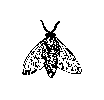
\epsfig{file=fly.eps}
\caption{A sample black and white graphic (.eps format).}
\end{figure}

\begin{figure}
\centering
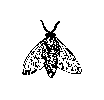
\epsfig{file=fly.eps, height=1in, width=1in}
\caption{A sample black and white graphic (.eps format)
that has been resized with the \texttt{epsfig} command.}
\end{figure}


As was the case with tables, you may want a figure
that spans two columns.  To do this, and still to
ensure proper ``floating'' placement of tables, use the environment
\textbf{figure*} to enclose the figure and its caption.
and don't forget to end the environment with
{figure*}, not {figure}!

\begin{figure*}
\centering
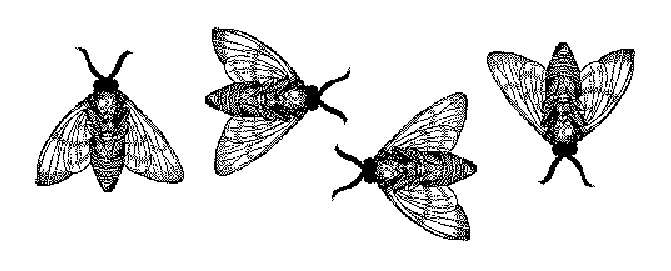
\epsfig{file=flies.eps}
\caption{A sample black and white graphic (.eps format)
that needs to span two columns of text.}
\end{figure*}

Note that either {\textbf{.ps}} or {\textbf{.eps}} formats are
used; use
the \texttt{{\char'134}epsfig} or \texttt{{\char'134}psfig}
commands as appropriate for the different file types.


\subsection{Theorem-like Constructs}
Other common constructs that may occur in your article are
the forms for logical constructs like theorems, axioms,
corollaries and proofs.  There are
two forms, one produced by the
command \texttt{{\char'134}newtheorem} and the
other by the command \texttt{{\char'134}newdef}; perhaps
the clearest and easiest way to distinguish them is
to compare the two in the output of this sample document:

This uses the \textbf{theorem} environment, created by
the\linebreak\texttt{{\char'134}newtheorem} command:
\newtheorem{theorem}{Theorem}
\begin{theorem}
Let $f$ be continuous on $[a,b]$.  If $G$ is
an antiderivative for $f$ on $[a,b]$, then
\begin{displaymath}\int^b_af(t)dt = G(b) - G(a).\end{displaymath}
\end{theorem}

The other uses the \textbf{definition} environment, created
by the \texttt{{\char'134}newdef} command:
\newdef{definition}{Definition}
\begin{definition}
If $z$ is irrational, then by $e^z$ we mean the
unique number which has
logarithm $z$: \begin{displaymath}{\log e^z = z}\end{displaymath}
\end{definition}

Two lists of constructs that use one of these
forms is given in the
\textit{Author's  Guidelines}.
 
There is one other similar construct environment, which is
already set up
for you; i.e. you must \textit{not} use
a \texttt{{\char'134}newdef} command to
create it: the \textbf{proof} environment.  Here
is a example of its use:
\begin{proof}
Suppose on the contrary there exists a real number $L$ such that
\begin{displaymath}
\lim_{x\rightarrow\infty} \frac{f(x)}{g(x)} = L.
\end{displaymath}
Then
\begin{displaymath}
l=\lim_{x\rightarrow c} f(x)
= \lim_{x\rightarrow c}
\left[ g{x} \cdot \frac{f(x)}{g(x)} \right ]
= \lim_{x\rightarrow c} g(x) \cdot \lim_{x\rightarrow c}
\frac{f(x)}{g(x)} = 0\cdot L = 0,
\end{displaymath}
which contradicts our assumption that $l\neq 0$.
\end{proof}

Complete rules about using these environments and using the
two different creation commands are in the
\textit{Author's Guide}; please consult it for more
detailed instructions.  If you need to use another construct,
not listed therein, which you want to have the same
formatting as the Theorem
or the Definition\cite{salas:calculus} shown above,
use the \texttt{{\char'134}newtheorem} or the
\texttt{{\char'134}newdef} command,
respectively, to create it.

\subsection*{A {\secit Caveat} for the \TeX\ Expert}
Because you have just been given permission to
use the \texttt{{\char'134}newdef} command to create a
new form, you might think you can
use \TeX's \texttt{{\char'134}def} to create a
new command: \textit{Please refrain from doing this!}
Remember that your \LaTeX\ source code is primarily intended
to create camera-ready copy, but may be converted
to other forms -- e.g. HTML. If you inadvertently omit
some or all of the \texttt{{\char'134}def}s recompilation will
be, to say the least, problematic.

\section{Conclusions}
This paragraph will end the body of this sample document.
Remember that you might still have Acknowledgments or
Appendices; brief samples of these
follow.  There is still the Bibliography to deal with; and
we will make a disclaimer about that here: with the exception
of the reference to the \LaTeX\ book, the citations in
this paper are to articles which have nothing to
do with the present subject and are used as
examples only.
%\end{document}  % This is where a 'short' article might terminate

%ACKNOWLEDGMENTS are optional
\section{Acknowledgments}
This section is optional; it is a location for you
to acknowledge grants, funding, editing assistance and
what have you.  In the present case, for example, the
authors would like to thank Gerald Murray of ACM for
his help in codifying this \textit{Author's Guide}
and the \textbf{.cls} and \textbf{.tex} files that it describes.

%
% The following two commands are all you need in the
% initial runs of your .tex file to
% produce the bibliography for the citations in your paper.
\bibliographystyle{abbrv}
\bibliography{sigproc}  % sigproc.bib is the name of the Bibliography in this case
% You must have a proper ".bib" file
%  and remember to run:
% latex bibtex latex latex
% to resolve all references
%
% ACM needs 'a single self-contained file'!
%
%APPENDICES are optional
%\balancecolumns
\appendix
%Appendix A
\section{Headings in Appendices}
The rules about hierarchical headings discussed above for
the body of the article are different in the appendices.
In the \textbf{appendix} environment, the command
\textbf{section} is used to
indicate the start of each Appendix, with alphabetic order
designation (i.e. the first is A, the second B, etc.) and
a title (if you include one).  So, if you need
hierarchical structure
\textit{within} an Appendix, start with \textbf{subsection} as the
highest level. Here is an outline of the body of this
document in Appendix-appropriate form:
\subsection{Introduction}
\subsection{The Body of the Paper}
\subsubsection{Type Changes and  Special Characters}
\subsubsection{Math Equations}
\paragraph{Inline (In-text) Equations}
\paragraph{Display Equations}
\subsubsection{Citations}
\subsubsection{Tables}
\subsubsection{Figures}
\subsubsection{Theorem-like Constructs}
\subsubsection*{A Caveat for the \TeX\ Expert}
\subsection{Conclusions}
\subsection{Acknowledgments}
\subsection{Additional Authors}
This section is inserted by \LaTeX; you do not insert it.
You just add the names and information in the
\texttt{{\char'134}additionalauthors} command at the start
of the document.
\subsection{References}
Generated by bibtex from your ~.bib file.  Run latex,
then bibtex, then latex twice (to resolve references)
to create the ~.bbl file.  Insert that ~.bbl file into
the .tex source file and comment out
the command \texttt{{\char'134}thebibliography}.
% This next section command marks the start of
% Appendix B, and does not continue the present hierarchy
\section{More Help for the Hardy}
The sig-alternate.cls file itself is chock-full of succinct
and helpful comments.  If you consider yourself a moderately
experienced to expert user of \LaTeX, you may find reading
it useful but please remember not to change it.
%\balancecolumns % GM June 2007
% That's all folks!
\end{document}
